\documentclass[
11pt, % The default document font size, options: 10pt, 11pt, 12pt
%codirector, % Uncomment to add a codirector to the title page
]{charter}


% El títulos de la memoria, se usa en la carátula y se puede usar el cualquier lugar del documento con el comando \ttitle
\titulo{Desarrollo de un collar inteligente para mascotas basado en tecnologías de geolocalización y redes celulares}

% Nombre del posgrado, se usa en la carátula y se puede usar el cualquier lugar del documento con el comando \degreename
\posgrado{Carrera de Especialización en Sistemas Embebidos}

% Tu nombre, se puede usar el cualquier lugar del documento con el comando \authorname
% IMPORTANTE: no omitir titulaciones ni tildación en los nombres, también se recomienda escribir los nombres completos (tal cual los tienen en su documento)
\autor{Ing. Joaquin Restovich}

% El nombre del director y co-director, se puede usar el cualquier lugar del documento con el comando \supname y \cosupname y \pertesupname y \pertecosupname
\director{Esp. Ing. Gonzalo Sanchez}
\pertenenciaDirector{FIUBA}
\codirector{} % para que aparezca en la portada se debe descomentar la opción codirector en los parámetros de documentclass
\pertenenciaCoDirector{FIUBA}

% Nombre del cliente, quien va a aprobar los resultados del proyecto, se puede usar con el comando \clientename y \empclientename
\cliente{Ing. Renata Gola}
\empresaCliente{Usuario final}

\fechaINICIO{28 de abril de 2026}		%Fecha de inicio de la cursada de GdP \fechaInicioName
\fechaFINALPlan{16 de junio de 2026} 	%Fecha de final de cursada de GdP
\fechaFINALTrabajo{junio de 2027}	%Fecha de defensa pública del trabajo final

\usepackage{xltabular}

% Fuerza los nombres automáticos de figuras en español.
\AtBeginDocument{%
  \selectlanguage{spanish}%
  \renewcommand{\figurename}{Figura}%
}

\begin{document}

\maketitle
\thispagestyle{empty}
\pagebreak


\thispagestyle{empty}
{\setlength{\parskip}{0pt}
\tableofcontents{}
}
\pagebreak


\section*{Registros de cambios}
\label{sec:registro}


\begin{table}[ht]
\label{tab:registro}
\centering
\begin{tabularx}{\linewidth}{@{}|c|X|c|@{}}
\hline
\rowcolor[HTML]{C0C0C0}
Revisión & \multicolumn{1}{c|}{\cellcolor[HTML]{C0C0C0}Detalles de los cambios realizados} & Fecha      \\ \hline
0      & Creación del documento                                                             & \fechaInicioName \\ \hline
1      & Se completa hasta el punto 5 inclusive                                             & 13 de mayo de 2026 \\ \hline
2      & Se completa hasta el punto 9 inclusive                                             & 17 de mayo de 2026 \\ \hline
3      & Reestructuración del documento para adecuarlo al formato de la plantilla oficial   & 17 de mayo de 2026 \\ \hline
4      & Se completa hasta el punto 12 inclusive                							& 24 de mayo de 2026 \\ \hline
5	   & Se completa el plan	                                 							& 01 de junio de 2026 \\ \hline
\end{tabularx}
\end{table}

\pagebreak


\section*{Acta de constitución del proyecto}
\label{sec:acta}

\begin{flushright}
Buenos Aires, \fechaInicioName
\end{flushright}

\vspace{2cm}

Por medio de la presente se acuerda con el \authorname\hspace{1px} que su Trabajo Final de la \degreename\hspace{1px} se titulará ``\ttitle'' y consistirá en la implementación de un prototipo de un collar rastreador de mascotas. El trabajo tendrá un presupuesto preliminar estimado de 600 horas y un costo estimado de USD 600, con fecha de inicio el \fechaInicioName\hspace{1px} y fecha de presentación pública en \fechaFinalName.

Se adjunta a esta acta la planificación inicial.

\vfill

% Esta parte se construye sola con la información que hayan cargado en el preámbulo del documento y no debe modificarla
\begin{table}[ht]
\centering
\begin{tabular}{ccc}
\begin{tabular}[c]{@{}c@{}}Dr. Ing. Ariel Lutenberg \\ Director posgrado FIUBA\end{tabular} & \hspace{2cm} & \begin{tabular}[c]{@{}c@{}}\clientename \\ Cliente \end{tabular} \vspace{2.5cm} \\
\multicolumn{3}{c}{\begin{tabular}[c]{@{}c@{}} \supname \\ Director del Trabajo Final\end{tabular}} \vspace{2.5cm} \\
\end{tabular}
\end{table}


\section{1. Descripción técnica-conceptual del proyecto a realizar}
\label{sec:descripcion}

El proyecto nace de una situación frecuente y angustiante para muchos dueños de mascotas: el extravío o escape del animal. En esos casos, la incertidumbre sobre su ubicación y la falta de herramientas accesibles para iniciar una búsqueda rápida vuelven especialmente valiosa la posibilidad de contar con asistencia tecnológica. A partir de esta problemática se propone el desarrollo de un prototipo de collar inteligente que incorpore geolocalización mediante GPS y conectividad celular para reportar su posición.

Actualmente existen productos similares en el mercado internacional, pero no logran ofrecer una propuesta del todo adecuada para el contexto local. Por un lado, hay alternativas importadas con costos iniciales altos o con suscripciones mensuales dolarizadas, como Tractive o ComfyTracker(TM). Por otro lado, también existen soluciones basadas en dispositivos auxiliares como AirTag, cuyo funcionamiento depende del ecosistema Apple tanto para la detección del dispositivo como para su posterior localización. Ninguna de estas opciones está especialmente orientada al mercado argentino, ni contempla de forma integral sus restricciones económicas y operativas.

El objetivo del proyecto es brindar una respuesta a esta problemática mediante una solución nacional, con disponibilidad local, soporte cercano y un costo competitivo. El alcance de este trabajo se concentra en el desarrollo de un prototipo funcional basado en una placa de desarrollo. El proyecto comprende el firmware necesario, la integración con periféricos externos y un dashboard básico para interactuar con el dispositivo. El desarrollo de una placa de hardware dedicada y de una aplicación móvil queda previsto para etapas posteriores.

Se trata de un proyecto de índole personal, con la posibilidad de evolucionar a una fase comercial futura si se obtiene financiamiento y si los costos del producto resultan competitivos para el mercado objetivo. El usuario al que apunta la solución está conformado por personas que consideran a sus mascotas parte de su familia y que están dispuestas a adquirir un dispositivo que permita encontrarlas rápidamente en caso de extravío o robo. Para que la propuesta sea atractiva, el producto debe ser accesible y sostener un esquema de uso simple, donde el único costo recurrente sea un abono de conectividad celular análogo al de un teléfono.

Uno de los principales desafíos del proyecto consiste en encontrar un equilibrio adecuado entre autonomía, funcionalidad y costo. Será necesario diseñar un dispositivo con suficiente duración de batería para operar durante períodos prolongados, garantizar cobertura celular en distintos entornos y mantener un tamaño y peso reducidos para no afectar la comodidad del animal. A esto se suma la necesidad de brindar robustez frente al uso diario y de alcanzar un costo final que permita una adopción amplia.

En la figura \ref{fig:diagBloques} se presenta el diagrama en bloques del sistema propuesto. Allí se observan los principales subsistemas del prototipo: un módulo GPS para la geolocalización, un módulo 4G para la transmisión remota de datos, una tarjeta SD para almacenamiento local ante pérdidas de conectividad, un LED de estado como interfaz mínima con el usuario y una batería como fuente de alimentación del conjunto.

\begin{figure}[htpb]
\centering
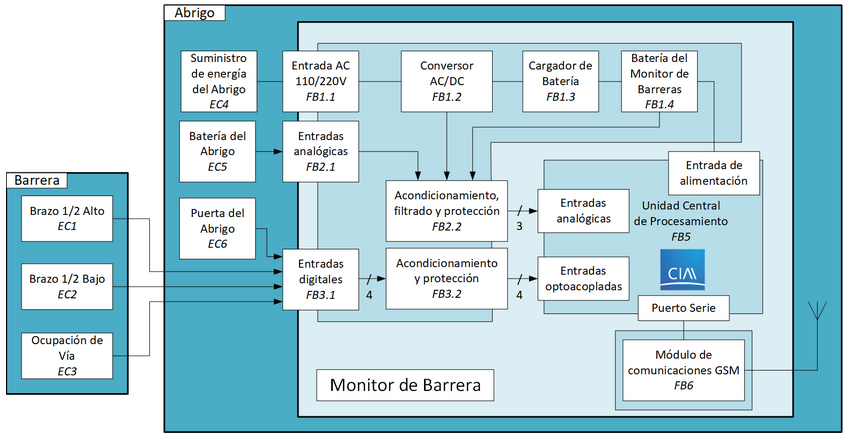
\includegraphics[width=.65\textwidth]{./Figuras/diagBloques.png}
\caption{Diagrama en bloques del sistema propuesto.}
\label{fig:diagBloques}
\end{figure}


\section{2. Identificación y análisis de los interesados}
\label{sec:interesados}

\begin{table}[ht]
\begin{tabularx}{\linewidth}{@{}|l|X|X|l|@{}}
\hline
\rowcolor[HTML]{C0C0C0}
Rol           & Nombre y Apellido & Organización      & Puesto                      \\ \hline
Cliente       & \clientename      & \empclientename   & Usuarios objetivo           \\ \hline
Responsable   & \authorname       & FIUBA             & Alumno                      \\ \hline
Orientador    & \supname          & \pertesupname     & Director del Trabajo Final  \\ \hline
Usuario final & Dueños de mascotas & -                & Usuario del sistema         \\ \hline
\end{tabularx}
\end{table}

\begin{itemize}
	\item Cliente: la Ing. Renata Gorla será el cliente, comprometiendose a evaluar la propuesta de valor del proyecto y dar su feedback en las diferentes versiones del prototipo. Su principal interés es contar con una solución confiable, simple de usar y con un costo de adquisición y mantenimiento accesible.
	\item Responsable: Joaquin Restovich es quien define, implementa e integra los distintos componentes del prototipo, además de planificar las tareas y verificar el cumplimiento de los objetivos del proyecto.
	\item Orientador: el Esp. Ing. Gonzalo Sanchez brindará guía técnica y metodológica para ayudar en la revisión del enfoque general, la definición de prioridades y la validación de las decisiones de diseño.
	\item Usuario final: los dueños de mascotas utilizarán el sistema para localizar a sus animales en caso de extravío. Se espera que valoren especialmente la facilidad de uso, la autonomía del dispositivo y la disponibilidad de la información de ubicación.
\end{itemize}


\section{3. Propósito del proyecto}
\label{sec:proposito}

Brindar una solución accesible para localizar mascotas extraviadas de manera rápida y confiable, mediante el desarrollo y validación de un prototipo con GPS y conectividad 4G que permita comprobar su viabilidad técnica y sentar las bases para una futura solución orientada al mercado local.


\section{4. Alcance del proyecto}
\label{sec:alcance}

El proyecto incluye:
\begin{itemize}
	\item Selección de componentes principales del sistema.
	\begin{itemize}
		\item Selección de microcontrolador o plataforma de desarrollo.
		\item Selección de batería y sistema de carga.
		\item Selección de módulo GPS.
		\item Selección de módulo 4G.
		\item Selección de memoria microSD.
	\end{itemize}
	\item Diseño de la arquitectura del firmware e integración de módulos periféricos.
	\item Desarrollo del firmware del prototipo.
	\begin{itemize}
		\item Módulo de control de batería.
		\item Módulo de adquisición y procesamiento de datos GPS.
		\item Módulo de comunicación 4G.
		\item Módulo de comunicación MQTT.
		\item Módulo de control del LED de estado.
		\item Módulo de almacenamiento en tarjeta SD.
	\end{itemize}
	\item Diseño e implementación de un dashboard básico para visualizar el estado del dispositivo y su ubicación.
	\item Selección y configuración de un broker MQTT.
	\item Pruebas de integración y pruebas de campo del prototipo.
\end{itemize}

El presente proyecto no incluye:
\begin{itemize}
	\item Desarrollo de hardware dedicado.
	\item Desarrollo de una aplicación móvil nativa.
	\item Diseño mecánico o carcasa plástica definitiva.
	\item Certificación regulatoria o habilitación comercial del dispositivo.
	\item Diseño de PCB definitivo.
\end{itemize}


\section{5. Supuestos del proyecto}
\label{sec:supuestos}

Para el desarrollo del presente proyecto se supone que:
\begin{itemize}
	\item El proyecto tendrá una duración del orden de 600 horas de ingeniería.
	\item Los componentes de hardware necesarios podrán adquirirse dentro de un presupuesto de hasta USD 500, sin restricciones de importación que alteren significativamente los costos estimados.
	\item La adquisición de componentes podrá realizarse en los plazos requeridos para sostener la planificación del proyecto.
	\item Las herramientas y plataformas de desarrollo necesarias estarán disponibles y serán técnicamente compatibles entre sí.
	\item La cobertura de red 4G en la zona de pruebas será suficiente para validar la conectividad del dispositivo.
	\item Los módulos GPS y 4G seleccionados contarán con documentación técnica y soporte de la comunidad adecuados para el desarrollo.
\end{itemize}


\section{6. Requerimientos}
\label{sec:requerimientos}

\begin{enumerate}
	\item Requerimientos funcionales:
	\begin{enumerate}
		\item El sistema debe adquirir periódicamente la ubicación geográfica del collar mediante un módulo GPS.
		\item El sistema debe transmitir la ubicación y el estado general del dispositivo a través de una red celular 4G.
		\item El sistema debe enviar la información remota utilizando MQTT como protocolo de mensajería.
		\item El sistema debe almacenar temporalmente la información en una memoria microSD cuando no haya conectividad y reportarla una vez restablecida la comunicación.
		\item El sistema debe informar el estado general del dispositivo mediante un LED local y mediante datos visibles en un dashboard remoto.
		\item El sistema debe permitir visualizar la última ubicación reportada, el estado de conectividad y el nivel de batería desde una interfaz accesible por navegador.
	\end{enumerate}
	
	\item Requerimientos de diseño e integración:
	\begin{enumerate}
		\item El prototipo debe implementarse sobre una plataforma de desarrollo, sin requerir hardware dedicado en esta etapa.
		\item El sistema debe integrar, como mínimo, los módulos GPS, 4G, batería, memoria microSD y una interfaz básica de estado.
		\item El dispositivo debe mantener dimensiones y peso compatibles con el uso en una mascota, procurando un peso menor a 200g y dimensaciones que no exederan los 80 x 60 x 30 mm.
	\end{enumerate}
	
	\item Requerimientos de validación:
	\begin{enumerate}
		\item Se realizarán pruebas unitarias de los componentes principales de firmware.
		\item La solución debe ser validada mediante pruebas de integración y al menos una prueba de campo.
		\item La precisión de ubicación y la transmisión remota deben contrastarse con mediciones o referencias conocidas.
		\item La autonomía del prototipo debe resultar suficiente para ejecutar los ensayos definidos para el proyecto.
	\end{enumerate}
	
	\item Requerimientos de documentación:
	\begin{enumerate}
		\item El proyecto debe incluir la memoria técnica del trabajo final.
		\item El proyecto debe contar con la documentación técnica del firmware siguiendo el formato doxygen.
		\item El proyecto debe contar con la documentación técnica del dashboard.
	\end{enumerate}
\end{enumerate}


\section{7. Historias de usuarios (\textit{Product backlog})}
\label{sec:backlog}

En esta sección se presentan las épicas principales del proyecto y las historias de usuario asociadas, organizadas según los roles de cliente, responsable del proyecto y usuario final. Las historias de usuario permiten describir las funcionalidades esperadas del sistema expresando quién requiere una determinada capacidad, qué necesita y con qué propósito.

Para estimar el tamaño relativo de cada historia de usuario se utilizará una ponderación en \textit{Story Points}. La estimación se realizará en función de tres aspectos: dificultad, complejidad y riesgo. Para cada uno de ellos se adoptará una escala basada en la serie de Fibonacci.

\begin{itemize}
	\item \textbf{Dificultad}: baja 1 punto, media 2 puntos, alta 5 puntos.
	\item \textbf{Complejidad}: baja 1 punto, media 3 puntos, alta 5 puntos.
	\item \textbf{Riesgo}: bajo 1 punto, medio 2 puntos, alto 3 puntos.
\end{itemize}

Los valores finales posibles de \textit{Story Points} serán: 1, 2, 3, 5, 8 y 13.

\begin{itemize}
	\item \textbf{Épica 1: adquisición de ubicación de la mascota}
	\begin{itemize}
		\item \textbf{HU1:} como usuario final, quiero que el collar obtenga la geolocalización de mi mascota mediante GPS para recuperarla en caso de extravío.\\
		Prioridad: Alta. \textit{Story Points}: 8.
		\item \textbf{HU2:} como responsable del proyecto, quiero integrar un módulo GPS en el sistema para disponer de la ubicación del dispositivo para su posterior reporte.\\
		Prioridad: Alta. \textit{Story Points}: 13.
	\end{itemize}
	\item \textbf{Épica 2: comunicación remota de la información}
	\begin{itemize}
		\item \textbf{HU3:} como usuario final, quiero que el collar envíe la ubicación de la mascota a través de la red celular para poder consultarla de manera remota.\\
		Prioridad: Alta. \textit{Story Points}: 13.
		\item \textbf{HU4:} como responsable del proyecto, quiero implementar la comunicación entre el dispositivo y el sistema remoto mediante la red 4G y el protocolo MQTT para transmitir de forma confiable la información al dashboard.\\
		Prioridad: Alta. \textit{Story Points}: 8.
	\end{itemize}
	\item \textbf{Épica 3: operación autónoma y confiable del dispositivo}
	\begin{itemize}
		\item \textbf{HU5:} como cliente, quiero que el prototipo tenga autonomía suficiente para validar su viabilidad como solución utilizable en condiciones reales.\\
		Prioridad: Alta. \textit{Story Points}: 8.
		\item \textbf{HU6:} como usuario final, quiero conocer el estado general del collar para saber el estado del mismo. Esta información me permitirá tomar deciciones como cargar la batería, detectar un fallo del dispositivo o buscar a mi mascota.\\
		Prioridad: Media. \textit{Story Points}: 3.
	\end{itemize}
	\item \textbf{Épica 4: visualización e interacción con el sistema}
	\begin{itemize}
		\item \textbf{HU7:} como usuario final, quiero visualizar la última ubicación reportada del collar para encontrar a mi mascota de manera rápida y sencilla.\\
		Prioridad: Alta. \textit{Story Points}: 8.
		\item \textbf{HU8:} como cliente, quiero disponer de un dashboard con información de ubicación y estado del dispositivo para evaluar el funcionamiento integral del prototipo.\\
		Prioridad: Media. \textit{Story Points}: 5.
	\end{itemize}
\end{itemize}

\subsection*{Criterios de aceptación}

\begin{itemize}
	\item \textbf{HU1}
	\begin{itemize}
		\item Validar la ubicación de GPS tomando como referencia otros puntos conocidos.
		\item La posición de GPS debe tener una precisión y convergencia adecuadas para localizar el collar de manera efectiva.
		\item Ante un fallo del módulo GPS se debe informar de forma fehaciente al usuario sobre esta situación.
	\end{itemize}
	\item \textbf{HU2}
	\begin{itemize}
		\item El firmware debe inicializar el módulo GPS al arrancar el sistema.
		\item El sistema debe comunicarse con el módulo GPS y ser capaz de interpretar las tramas entregadas por el módulo.
		\item Ante pérdida de señal o mal funcionamiento del módulo GPS, el sistema debe proteger el resto de las funcionalidades.
	\end{itemize}
	\item \textbf{HU3}
	\begin{itemize}
		\item Se debe corroborar la conexión del dispositivo a la red celular.
		\item Se debe corroborar la conexión del dispositivo con el broker en la nube.
		\item La información transmitida debe incluir un identificador del dispositivo, las coordenadas y la marca temporal.
	\end{itemize}
	\item \textbf{HU4}
	\begin{itemize}
		\item Se debe corroborar la conexión al broker MQTT.
		\item Se deben definir los tópicos y la forma de codificar la información.
		\item El dispositivo debe publicar los mensajes en los tópicos correspondientes.
		\item Ante una desconexión de red o del broker, el sistema debe intentar reconectarse automáticamente.
	\end{itemize}
	\item \textbf{HU5}
	\begin{itemize}
		\item El prototipo debe operar durante el período mínimo de autonomía definido para la prueba de campo.
		\item El sistema debe alimentarse únicamente desde la batería prevista durante la prueba de autonomía, partiendo de un estado con 100\% de carga.
		\item Durante la prueba no deben producirse reinicios inesperados ni pérdida total de funcionalidad.
	\end{itemize}
	\item \textbf{HU6}
	\begin{itemize}
		\item El sistema debe informar el estado de batería.
		\item El sistema debe informar el estado del módulo GPS y el estado general del sistema.
		\item Ante períodos de desconexión de la red 4G o del broker MQTT, se debe registrar e informar la situación al recuperarse la conectividad.
		\item La última ubicación disponible del dispositivo debe poder consultarse junto con su estado general.
	\end{itemize}
	\item \textbf{HU7}
	\begin{itemize}
		\item El dashboard debe mostrar la última ubicación recibida del dispositivo.
		\item La visualización debe incluir la fecha y hora del último reporte.
		\item Si no hay datos luego de un tiempo definido, el dashboard debe indicar claramente que la información no está actualizada.
	\end{itemize}
	\item \textbf{HU8}
	\begin{itemize}
		\item El dashboard debe mostrar al menos ubicación, estado de conectividad y nivel de batería.
		\item El dashboard debe permitir verificar que la cadena completa de adquisición, transmisión y visualización funciona correctamente.
		\item La información del dispositivo debe presentarse en una interfaz accesible desde navegador.
	\end{itemize}
\end{itemize}


\section{8. Entregables principales del proyecto}
\label{sec:entregables}

Los entregables principales del proyecto son:
\begin{itemize}
	\item Documento de selección de componentes principales del prototipo.
	\item Diagrama en bloques de la solución.
	\item Firmware fuente del sistema embebido.
	\item Configuración de comunicación 4G y MQTT.
	\item Dashboard básico para visualización de ubicación y estado del dispositivo.
	\item Registro de pruebas de integración y pruebas de campo.
	\item Documentación técnica del prototipo desarrollado.
	\item Memoria del trabajo final.
\end{itemize}


\section{9. Desglose del trabajo en tareas}
\label{sec:wbs}

El desglose preliminar del trabajo se organiza de la siguiente forma:

\begin{enumerate}
\item Planificación y definición del proyecto (60 h)
	\begin{enumerate}
	\item Relevamiento del problema y del estado del arte (15 h)
	\item Definición de alcance, supuestos y requerimientos (15 h)
	\item Elaboración del backlog y criterios de aceptación (15 h)
	\item Planificación general del proyecto y estimación de esfuerzo (15 h)
	\end{enumerate}
\item Selección e integración de hardware (120 h)
	\begin{enumerate}
	\item Selección de plataforma de desarrollo y microcontrolador (20 h)
	\item Selección del módulo GPS (20 h)
	\item Selección del módulo 4G y plan de datos para pruebas (20 h)
	\item Selección de batería, sistema de carga y protecciones (20 h)
	\item Integración física inicial de los módulos del prototipo (20 h)
	\item Verificación eléctrica y funcional básica del conjunto (20 h)
	\end{enumerate}
\item Desarrollo del firmware embebido (170 h)
	\begin{enumerate}
	\item Arquitectura de software y definición de módulos (30 h)
	\item Desarrollo del módulo de adquisición GPS (30 h)
	\item Desarrollo del módulo de comunicación 4G (30 h)
	\item Desarrollo del módulo MQTT (30 h)
	\item Desarrollo del manejo de almacenamiento en microSD (20 h)
	\item Desarrollo del control de batería y gestión de energía (20 h)
	\item Desarrollo del módulo de LED de estado y diagnóstico básico (10 h)
	\end{enumerate}
\item Desarrollo del sistema remoto y visualización (90 h)
	\begin{enumerate}
	\item Selección y configuración del broker MQTT (20 h)
	\item Definición del formato de mensajes y tópicos (15 h)
	\item Diseño del dashboard de monitoreo (20 h)
	\item Implementación del dashboard básico (35 h)
	\end{enumerate}
\item Validación del prototipo (80 h)
	\begin{enumerate}
	\item Pruebas unitarias e integración entre módulos (20 h)
	\item Pruebas de conectividad celular y transmisión remota (20 h)
	\item Pruebas de almacenamiento local ante pérdida de conectividad (20 h)
	\item Pruebas de campo de geolocalización y autonomía (20 h)
	\end{enumerate}
\item Documentación y cierre (80 h)
	\begin{enumerate}
	\item Registro de resultados y análisis de ensayos (20 h)
	\item Redacción de la memoria técnica (30 h)
	\item Preparación de material de presentación y defensa (20 h)
	\item Ajustes finales y cierre del proyecto (10 h)
	\end{enumerate}
\end{enumerate}

Cantidad total de horas: 600 h.


\section{10. Diagrama de Activity On Node}
\label{sec:AoN}

El diagrama de \textit{Activity on Node} se armó a partir del WBS definido en la sección anterior. En la figura \ref{fig:AoN} se muestran las principales tareas del proyecto y sus relaciones de precedencia. Los tiempos indicados en el diagrama están expresados en horas. Las flechas mas gruesas en ell diagrama contemplan las actividades involucradas en el camino crítico del proyecto.

\begin{landscape}
\begin{figure}[p]
\centering
\makebox[\linewidth][c]{%
  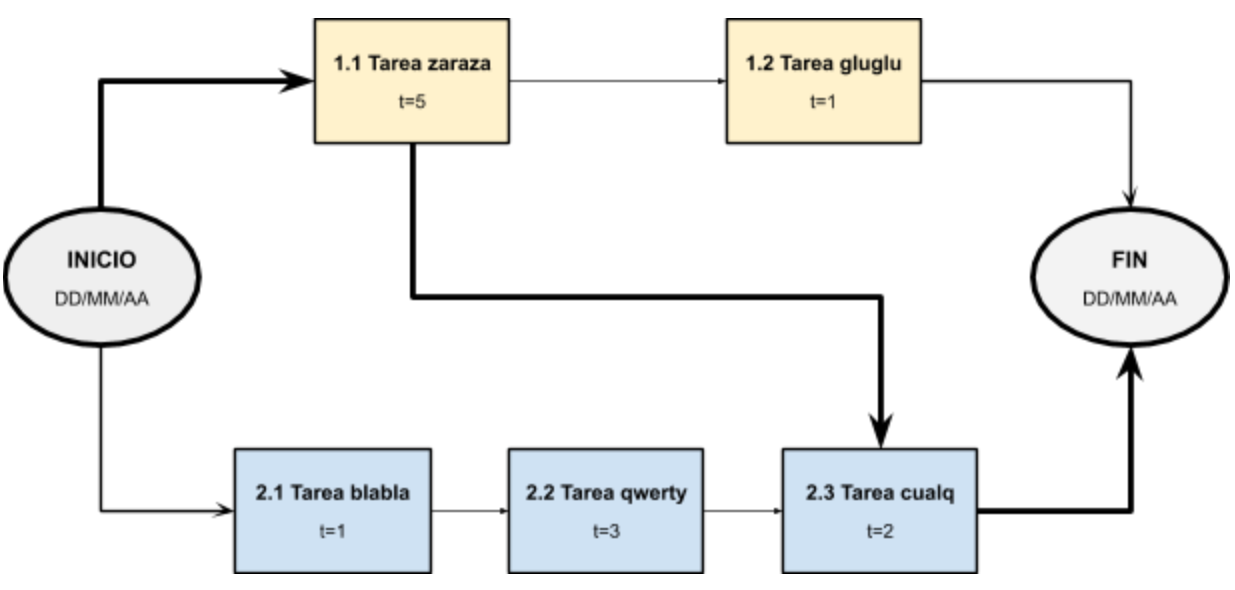
\includegraphics[width=1.02\linewidth,height=.74\textheight,keepaspectratio]{./Figuras/AoN.png}%
}
\caption{Diagrama de \textit{Activity on Node} del proyecto.}
\label{fig:AoN}
\end{figure}
\end{landscape}


\section{11. Diagrama de Gantt}
\label{sec:gantt}

A continuación se muestra una tabla con las fechas de inicio y fin de cada tarea y su carga en cantidad de horas. Además, en la figura \ref{fig:diagGantt} se presenta el diagrama de Gantt del proyecto. Este cronograma resume la distribución temporal de las actividades principales, muestra las tareas del EDT y deberá mantenerse consistente con la fecha de finalización indicada en el Acta Constitutiva.

\begin{table}[htpb]
\centering
\normalsize
\setlength{\tabcolsep}{2pt}
\renewcommand{\arraystretch}{0.88}
\begin{tabularx}{\linewidth}{@{}|C{0.8cm}|>{\raggedright\arraybackslash}X|C{1.9cm}|C{1.9cm}|C{1.6cm}|@{}}
\hline
\rowcolor[HTML]{C0C0C0}
ID & Actividad & \shortstack{Fecha de\\inicio} & \shortstack{Fecha de\\fin} & Duración \\ \hline
1 & Planificación y definición del proyecto & 1/11/27 & 1/29/27 & 15 \\ \hline
2 & Relevamiento del problema y del estado del arte & 1/11/27 & 1/14/27 & 4 \\ \hline
3 & Definición de alcance, supuestos y requerimientos & 1/15/27 & 1/20/27 & 4 \\ \hline
4 & Elaboración del backlog y criterios de aceptación & 1/21/27 & 1/25/27 & 3 \\ \hline
5 & Planificación general del proyecto y estimación de esfuerzo & 1/26/27 & 1/29/27 & 4 \\ \hline
6 & Selección e integración de hardware & 2/1/27 & 3/12/27 & 30 \\ \hline
7 & Selección de plataforma de desarrollo y microcontrolador & 2/1/27 & 2/5/27 & 5 \\ \hline
8 & Selección del módulo GPS & 2/8/27 & 2/12/27 & 5 \\ \hline
9 & Selección del módulo 4G y plan de datos para pruebas & 2/15/27 & 2/19/27 & 5 \\ \hline
10 & Selección de batería, sistema de carga y protecciones & 2/22/27 & 2/26/27 & 5 \\ \hline
11 & Integración física inicial de los módulos del prototipo & 3/1/27 & 3/5/27 & 5 \\ \hline
12 & Verificación eléctrica y funcional básica del conjunto & 3/8/27 & 3/12/27 & 5 \\ \hline
13 & Desarrollo del firmware embebido & 3/15/27 & 5/14/27 & 45 \\ \hline
14 & Arquitectura de software y definición de módulos & 3/15/27 & 3/24/27 & 8 \\ \hline
15 & Desarrollo del módulo de adquisición GPS & 3/25/27 & 4/5/27 & 8 \\ \hline
16 & Desarrollo del módulo de comunicación 4G & 4/6/27 & 4/15/27 & 8 \\ \hline
17 & Desarrollo del módulo MQTT & 4/26/27 & 5/5/27 & 8 \\ \hline
18 & Desarrollo del manejo de almacenamiento en microSD & 4/19/27 & 4/23/27 & 5 \\ \hline
19 & Desarrollo del control de batería y gestión de energía & 5/5/27 & 5/11/27 & 5 \\ \hline
20 & Desarrollo del módulo de LED de estado y diagnóstico básico & 5/12/27 & 5/14/27 & 3 \\ \hline
21 & Desarrollo del sistema remoto y visualización & 4/13/27 & 5/14/27 & 24 \\ \hline
22 & Selección y configuración del broker MQTT & 4/13/27 & 4/19/27 & 5 \\ \hline
23 & Definición del formato de mensajes y tópicos & 4/20/27 & 4/23/27 & 4 \\ \hline
24 & Diseño del dashboard de monitoreo & 4/27/27 & 5/3/27 & 5 \\ \hline
25 & Implementación del dashboard básico & 5/4/27 & 5/14/27 & 9 \\ \hline
26 & Validación del prototipo & 6/17/27 & 7/14/27 & 20 \\ \hline
27 & Pruebas unitarias e integración entre módulos & 6/17/27 & 6/23/27 & 5 \\ \hline
28 & Pruebas de conectividad celular y transmisión remota & 6/24/27 & 6/30/27 & 5 \\ \hline
29 & Pruebas de almacenamiento local ante pérdida de conectividad & 7/1/27 & 7/7/27 & 5 \\ \hline
30 & Pruebas de campo de geolocalización y autonomía & 7/8/27 & 7/14/27 & 5 \\ \hline
31 & Documentación y cierre & 7/15/27 & 8/12/27 & 21 \\ \hline
32 & Registro de resultados y análisis de ensayos & 7/15/27 & 7/21/27 & 5 \\ \hline
33 & Redacción de la memoria técnica & 7/22/27 & 8/2/27 & 8 \\ \hline
34 & Preparación de material de presentación y defensa & 8/3/27 & 8/9/27 & 5 \\ \hline
35 & Ajustes finales y cierre del proyecto & 8/10/27 & 8/12/27 & 3 \\ \hline

\end{tabularx}
\caption{Actividades consideradas para el diagrama de Gantt.}
\label{tab:gantt-actividades}
\end{table}

\clearpage
\begin{landscape}
\begin{figure}[p]
\centering
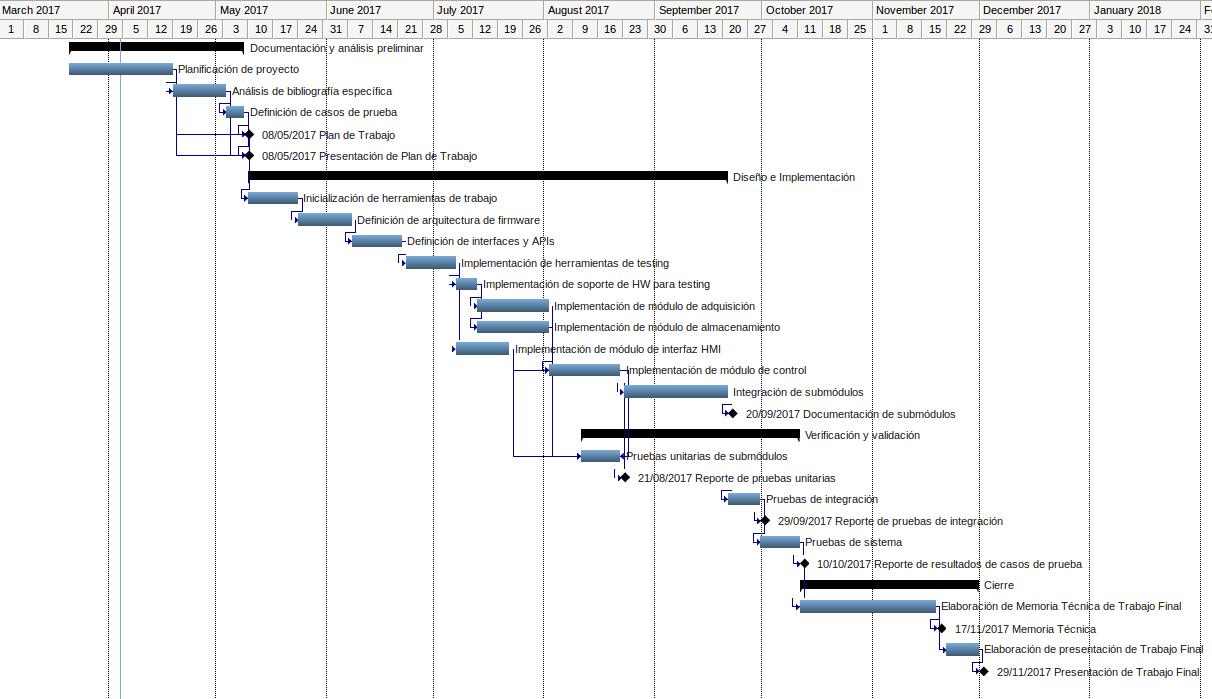
\includegraphics[height=.85\textheight]{./Figuras/Gantt-2.png}
\caption{Diagrama de Gantt del proyecto.}
\label{fig:diagGantt}
\end{figure}
\end{landscape}


\section{12. Presupuesto detallado del proyecto}
\label{sec:presupuesto}
El presupuesto detallado del proyecto se expresa en pesos argentinos. Para este proyecto se distinguen costos directos e indirectos. Dentro de los costos directos se considera los servicios profesionales de ingeniería, tomando como referencia el costo de la hora de ingeniería de un profesiona categoría semisenior publicado por COPITEC.

\begin{table}[htpb]
\centering
\begin{tabularx}{\linewidth}{@{}|X|c|r|r|@{}}
\hline
\rowcolor[HTML]{C0C0C0}
\multicolumn{4}{|c|}{\cellcolor[HTML]{C0C0C0}COSTOS DIRECTOS} \\ \hline
\rowcolor[HTML]{C0C0C0}
Descripción &
  \multicolumn{1}{c|}{\cellcolor[HTML]{C0C0C0}Cantidad} &
  \multicolumn{1}{c|}{\cellcolor[HTML]{C0C0C0}Valor unitario} &
  \multicolumn{1}{c|}{\cellcolor[HTML]{C0C0C0}Valor total} \\ \hline
Plataforma de desarrollo embebida &
  \multicolumn{1}{c|}{1} &
  \multicolumn{1}{c|}{\$ 6500} &
  \multicolumn{1}{c|}{\$ 6500} \\ \hline
Módulo GPS &
  \multicolumn{1}{c|}{1} &
  \multicolumn{1}{c|}{\$ 20000} &
  \multicolumn{1}{c|}{\$ 20000} \\ \hline
Módulo 4G &
  \multicolumn{1}{c|}{1} &
  \multicolumn{1}{c|}{\$ 58000} &
  \multicolumn{1}{c|}{\$ 58000} \\ \hline
Memoria microSD y adaptadores &
  \multicolumn{1}{c|}{1} &
  \multicolumn{1}{c|}{\$ 10000} &
  \multicolumn{1}{c|}{\$ 10000} \\ \hline
Batería, cargador y protecciones &
  \multicolumn{1}{c|}{1} &
  \multicolumn{1}{c|}{\$ 5000} &
  \multicolumn{1}{c|}{\$ 5000} \\ \hline
SIM y conectividad para pruebas &
  \multicolumn{1}{c|}{1} &
  \multicolumn{1}{c|}{\$ 5000} &
  \multicolumn{1}{c|}{\$ 5000} \\ \hline
Servicios profesionales &
  \multicolumn{1}{c|}{600} &
  \multicolumn{1}{c|}{\$ 150000} &
  \multicolumn{1}{c|}{\$ 90000000} \\ \hline
\multicolumn{3}{|c|}{SUBTOTAL} &
  \multicolumn{1}{c|}{\$ 90104500} \\ \hline
\rowcolor[HTML]{C0C0C0}
\multicolumn{4}{|c|}{\cellcolor[HTML]{C0C0C0}COSTOS INDIRECTOS} \\ \hline
\rowcolor[HTML]{C0C0C0}
Descripción &
  \multicolumn{1}{c|}{\cellcolor[HTML]{C0C0C0}Cantidad} &
  \multicolumn{1}{c|}{\cellcolor[HTML]{C0C0C0}Valor unitario} &
  \multicolumn{1}{c|}{\cellcolor[HTML]{C0C0C0}Valor total} \\ \hline
Reposición de componentes e imprevistos &
  \multicolumn{1}{c|}{1} &
  \multicolumn{1}{c|}{\$ 20000} &
  \multicolumn{1}{c|}{\$ 20000} \\ \hline
Amortización de herramientas y recursos auxiliares &
  \multicolumn{1}{c|}{1} &
  \multicolumn{1}{c|}{\$ 20000} &
  \multicolumn{1}{c|}{\$ 20000} \\ \hline
\multicolumn{3}{|c|}{SUBTOTAL} &
  \multicolumn{1}{c|}{\$ 40000} \\ \hline
\rowcolor[HTML]{C0C0C0}
\multicolumn{3}{|c|}{TOTAL} &
  \multicolumn{1}{c|}{\$ 90144500} \\ \hline
\end{tabularx}
\end{table}

\section{13. Gestión de riesgos}
\label{sec:riesgos}

Riesgo 1: dificultades en la importación de módulos.
\begin{itemize}
	\item Severidad (S): 8. No disponer de los componentes de hardware puede significar grandes demoras en el desaroolo del software, pudiendo ser un cuello de botella del desarrollo.
	\item Probabilidad de ocurrencia (O): 4. Luego de la seleccion de componentes se empezará con tareas que no requieran los componentes para intentar evitar tiempos muertos. LLegado el caso de sufir retrasos considerables en la importación se optará por provedores locales para el protoipo.
\end{itemize}

Riesgo 2: cobertura 4G insuficiente en los entornos de prueba.
\begin{itemize}
	\item Severidad (S): 7. Se deben analizar las zonas de cobertura de los diferentes provedores locales para asegurar que la correcta conexión del dispositivo y minimizar los posibles baches de cobertura.
	\item Probabilidad de ocurrencia (O): 4. Hoy en día la mayoria de provedores ofrecen buena cobertura en zonas urbanas.
\end{itemize}

Riesgo 3: autonomía del prototipo menor a la esperada.
\begin{itemize}
	\item Severidad (S): 9. El dimensionamiento de las baterías, el uso del modo de bajo consumo y la selección de módulos que consigan un correcto compromiso entre consumo y performance es clave para la viabilidad del proyecto, sin elevar significativamente los costos.
	\item Probabilidad de ocurrencia (O): 5.Se deben seleccionar con cuidado los componentes finales a utilizar.
\end{itemize}

Riesgo 4: dificultades de integración entre GPS, 4G y almacenamiento local.
\begin{itemize}
	\item Severidad (S): 7. Los diferentes módulso de firmware deben ser desarrollados de forma que puedan comunicarse entre ellos sin que esto represente una dificultad.
	\item Probabilidad de ocurrencia (O): 5. Se hará es desarrollo de una forma modular, haciendo test de cada uno de las partes para comprobar su correcto funcionamiento.
\end{itemize}

Riesgo 5: ensamblaje del prototipo.
\begin{itemize}
	\item Severidad (S): 6. Se debe lograr unir los diferentes módulos que componen el sistema de la forma mas compacta posible para que sea portable por una mascota.
	\item Probabilidad de ocurrencia (O): 6. al no contemplar el desarrollo de hardware dedicado es posible que los primero prototipos no sean tan compacto, haciendo que sean compatibles con mascotas de medianas a grandes.
\end{itemize}

A continuación se muestra la tabla de gestión de riesgos:

\begin{table}[htpb]
\centering
\begin{tabularx}{\linewidth}{@{}|X|c|c|c|c|c|c|@{}}
\hline
\rowcolor[HTML]{C0C0C0}
Riesgo & S & O & RPN & S* & O* & RPN* \\ \hline
Demoras en adquisición de módulos importados & 8 & 5 & 40 & 8 & 3 & 24 \\ \hline
Cobertura 4G insuficiente en pruebas & 7 & 4 & 28 & 7 & 4 & 28 \\ \hline
Autonomía menor a la esperada & 9 & 5 & 45 & 7 & 5 & 35 \\ \hline
Dificultades de integración entre subsistemas & 7 & 5 & 35 & 6 & 4 & 24 \\ \hline
Ensamblaje del prototipo & 6 & 6 & 36 & 5 & 5 & 25 \\ \hline
\end{tabularx}
\end{table}

Criterio adoptado:

Se tomarán medidas de mitigación en los riesgos cuyos números de RPN sean mayores o iguales a 36. Se toma esta valor como referencia tomando como referencia la situación en que la severidad y la probabilidad de ocurrencia tengan ambas un valos de 6.

Se presenta el siguiente plan de mitigación para intentar reducir los riesgos:

Riesgo 3 Mitigado: autonomía del prototipo menor a la esperada.
\begin{itemize}	
\item Severidad (S*): 7. Se medirá el consumo por subsistema y se ajustará la estrategia de transmisión y adquisición de datos para minimizar el consumo y maximizar la autonomía del dispositivo. Se optará por módulos que sean compatibles con las pretensiones energéticas del proyecto.
\item Probabilidad de ocurrencia (O*): 5. Se deben seleccionar con cuidado los componentes finales a utilizar.
\end{itemize}

Riesgo 5 Mitigado: ensamblaje del prototipo.
\begin{itemize}
\item Severidad (S*): 5. Para reducir el tamaño del protipo y asegurar la rigidez del mismo, se realizará un diseño con SolidWorks para contruir una carcasa impresa en 3D del prototipo. 
\item Probabilidad de ocurrencia (O*): 5. Se usará asesoria externa para optimizar el diseño físico.
\end{itemize}

\section{14. Gestión de la calidad}
\label{sec:calidad}

Se seleccionan a continuación diez requerimientos que, por su impacto en la funcionalidad principal, el desempeño del prototipo y el valor entregado al usuario, se consideran los más importantes del proyecto. Para cada uno se indican las acciones de verificación y validación que permitirán asegurar su cumplimiento.

\begin{itemize}
	\item Req. 1.1: el sistema debe adquirir periódicamente la ubicación geográfica del collar mediante un módulo GPS.
	\begin{itemize}
		\item Verificación estática: se tomarán la posición GPS en puntos conocidos duarante un tiempo de 5 minutos para verificar la precisión y la divergencia de la señal de GPS.
		\item Verificación dinámica: se tomarán la posición GPS en un recorrido conocidos para verificar la precisión y la divergencia de la señal de GPS.
		\item Validación estática: se realizará la comparación entre puntos GPS de referencia y la posición reportada por el dispositivo.
		\item Validación dinámica: se realizará la comparación entre el recorrido de GPS de realizado y el mismo recorrido tomado por un teléfono usando google maps.
	\end{itemize}

	\item Req. 1.2: el sistema debe transmitir la ubicación y el estado general del dispositivo a través de una red celular 4G.
	\begin{itemize}
		\item Verificación: Se comprobará la conexión del módulo a la red 4G haciendo un ping a una página conocida de referencia en puntos estáticos y en un recorrido .
		\item Validación: detallar la demostración al cliente en la que se confirme que la información llega en tiempo y forma adecuados para el uso esperado.
	\end{itemize}

	\item Req. 1.3: el sistema debe enviar la información remota utilizando MQTT como protocolo de mensajería.
	\begin{itemize}
		\item Verificación: Se harán pruebas d laboratorio sobre la conectividad al broker MQTT.
		\item Validación: se repetirán las verificaciones del req 1.1 pero esta vez logeando los fatos por MQTT.
	\end{itemize}

	\item Req. 1.4: el sistema debe almacenar temporalmente la información en una memoria microSD cuando no haya conectividad y reportarla una vez restablecida la comunicación.
	\begin{itemize}
		\item Verificación: emular escenarios donde se desconecta el módulo de 4g y verifificar que se guardan los datos en la memoria SD.
		\item Validación: Buscar zonas de falta se señal para probar el equipo en una situacion real.
	\end{itemize}

	\item Req. 1.5: el sistema debe informar el estado general del dispositivo mediante un LED local y mediante datos visibles en un dashboard remoto.
	\begin{itemize}
		\item Verificación: definir los diferentes estados del equipo y forzar el sistema a sus diferentes estados para comprobar la seãlización de cada uno de ellos.
		\item Validación: observar en forma visual el led de estado y verificar el estado en el broker MQTT.
	\end{itemize}

	\item Req. 1.6: el sistema debe permitir visualizar la última ubicación reportada, el estado de conectividad y el nivel de batería desde una interfaz accesible por navegador.
	\begin{itemize}
		\item Verificación: poder ver los datos del dispositivo en tiempo real, tanto en condiciones estáticas como dinámicas.
		\item Validación: comparar en tiempo real los datos generados por el dispositivos y por un celular usando google maps.
	\end{itemize}

	\item Req. 2.3: el dispositivo debe mantener dimensiones y peso compatibles con el uso en una mascota, procurando un peso menor a 200 g y dimensiones que no excedan los 80 x 60 x 30 mm.
	\begin{itemize}
		\item Verificación: detallar las mediciones físicas del prototipo, incluyendo peso, dimensiones y comparación contra los límites definidos.
		\item Validación: Pesar el sistema y definir una carcasa que contenga todos los módulos y cumpla las dimensiones
	\end{itemize}


	\item Req. 3.1. Se realizarán pruebas unitarias de los componentes principales de firmware.
	\begin{itemize}
		\item Verificación: definir un arnes de test y hacer pruebas de todos los módulos realizados y definir protocolos para validar cada uno de ellos.
		\item Validación: cobertura de al menos el 70\% de funcionalidades testeadas.
	\end{itemize}
	
	\item Req. 3.2: la solución debe ser validada mediante pruebas de integración y al menos una prueba de campo.
	\begin{itemize}
		\item Verificación: realizar pruebas de integración en laboratorio y pruebas en campo con el cliente.
		\item Validación: poder utilizar el dispositivo sin inconvenientes y recibir feedback del cliente.
	\end{itemize}

	\item Req. 3.4: la autonomía del prototipo debe resultar suficiente para ejecutar los ensayos definidos para el proyecto.
	\begin{itemize}
		\item Verificación: detallar las mediciones de consumo, cálculos de autonomía, ensayo de descarga en condiciones representativas y contraste con las hojas de datos de los componentes involucrados.
		\item Validación: detallar la confirmación con el cliente de que la duración obtenida satisface las expectativas mínimas para las pruebas y para el caso de uso considerado.
	\end{itemize}
\end{itemize}


\section{15. Procesos de cierre}
\label{sec:cierre}

Las pautas de trabajo para la reunión final de evaluación del proyecto contemplan las siguientes actividades:

\begin{itemize}
	\item Revisión del cumplimiento del plan original: 
	\begin{itemize}
		\item Responsable: Joaquin Restovich
		\item Procedimiento: Se analizará el cumplimiento con los requerimientos y cronograma
establecidos. En el caso de hallar requerimientos incumplidos y/o retrasos en las
tareas se evaluarán las causas y se propondrán acciones para evitarlo en futuros
proyectos.
	\end{itemize}

	\item Identificación de técnicas útiles, problemas encontrados y soluciones aplicadas:
	\begin{itemize}
		\item Responsable: Joaquin Restovich
		\item Procedimiento: Se evaluarán los procedimientos basándose en su utilidad
y eficiencia para alcanzar los objetivos predefinidos. Se analizarán los problemas
surgidos y las medidas paliativas.
	\end{itemize}
	
	\item Organización del cierre formal del proyecto y agradecimiento a los interesados: 
	\begin{itemize}
		\item Responsable: Joaquin Restovich
		\item  Se aprovechará la jornada de defensas organizada por el posgrado para realizar los agradecimientos formales a todos los interesados, colaboradores y personas que hayan
colaborado de alguna forma en el proyecto.
		\item Se preparará un mensaje de agradecimiento que reconozca el apoyo recibido y
destaque la importancia de cada colaborador en el éxito del proyecto.
		\item Financiamiento: Los gastos menores asociados a esta instancia serán asumidos dentro del presupuesto general del proyecto.
	\end{itemize}
\end{itemize}

\end{document}
